Given is the signal $s(t)$
\begin{figure}[H]
	\centering
	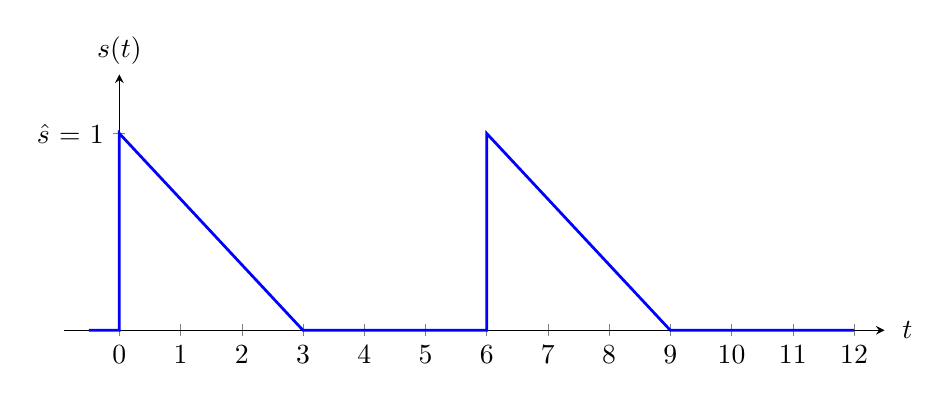
\begin{tikzpicture}
		\pgfplotsset{
			every axis plot/.append style={line width=1pt, mark=none}
		}
		\begin{axis}[
			clip=false,
			axis lines=middle,
			xmin=-0.9, xmax=12.5,
			xlabel={$t$},
			xtick distance={1},
			ymin=0, ymax=1.3,
			y=2.5cm,
			ylabel={$s(t)$},
			yticklabels={$\hat{s}$ = 1},
			ytick={1},
			width=12cm,
			x label style={at={(current axis.right of origin)},	anchor=east, right=1mm},
			y label style={at={(current axis.above origin)}, anchor=south },
			hide obscured x ticks=false
		]
			\addplot[color=blue] coordinates {(-0.5,0) (0,0) (0,1) (3,0) (6,0) (6,1) (9,0) (12,0)};
		\end{axis}
	\end{tikzpicture}
	\caption{\label{415}Periodic signal $s(t)$}
\end{figure}
\begin{enumerate}
	\item Formal description of the signal \newline
	The signal shown is periodic, with a period duration $T_0$ of 6 time units on $t$. 
	\begin{equation*}
		s(t) = s(t+n\cdot{T_0})
	\end{equation*}
	The following therefore applies:
	\begin{equation*}
		s(t+n\cdot{T_0}) = \begin{cases}
			1, \quad t = 0+6n \\
			\frac{1}{3}t + 1, \quad 0+6n < t < 3+6n \\
			0, \quad 3+6n < t \leq 6+6n
		\end{cases}
	\end{equation*}
	\clearpage
	\item Description and representation in Matlab
	\lstinputlisting[language=Matlab]{./assets/Lab1_415.m}
	{
		\setlength{\fboxsep}{0pt}%  
		\colorbox{backcolor}{\includegraphics[width=\linewidth, keepaspectratio]{./assets/415.png}}
	}
\end{enumerate}